% Template for ICIP-2015 paper; to be used with:
%          spconf.sty  - ICASSP/ICIP LaTeX style file, and
%          IEEEbib.bst - IEEE bibliography style file. cambio para probar
% --------------------------------------------------------------------------
\documentclass[spanish]{article}
\usepackage{spconf,amsmath,graphicx}
\usepackage{mathptmx}
\usepackage{mathtools}
\usepackage{amsmath}
\usepackage{mathrsfs}
\usepackage{amssymb}
\usepackage{amsfonts}
\usepackage[utf8]{inputenc}
\usepackage{babel}
\selectlanguage{spanish}
% Example definitions.
% --------------------
\def\x{{\mathbf x}}
\def\L{{\cal L}}

% Title.
% ------
\title{OPTIMIZACIÓN MULTIOBJETIVO PARA LA MEJORA DEL CONTRASTE BASADA EN CLAHE.}
%
% Single address.
% ---------------
\name{Author(s) Name(s)\thanks{Thanks to XYZ agency for funding.}}
\address{Author Affiliation(s)}
%
% For example:
% ------------
%\address{School\\
%	Department\\
%	Address}
%
% Two addresses (uncomment and modify for two-address case).
% ----------------------------------------------------------
%\twoauthors
%  {A. Author-one, B. Author-two\sthanks{Thanks to XYZ agency for funding.}}
%	{School A-B\\
%	Department A-B\\
%	Address A-B}
%  {C. Author-three, D. Author-four\sthanks{The fourth author performed the work
%	while at ...}}
%	{School C-D\\
%	Department C-D\\
%	Address C-D}
%
\begin{document}
%\ninept
%
\maketitle
%
\begin{abstract}
The abstract should appear at the top of the left-hand column of text, about
0.5 inch (12 mm) below the title area and no more than 3.125 inches (80 mm) in
length.  Leave a 12 mm (0.5 in.) space between the end of the abstract and the
beginning of the main text.  The abstract should contain about 100 to 150
words, and should be identical to the abstract text submitted electronically
along with the paper cover sheet.  All manuscripts must be in English, printed
in black ink.
\end{abstract}
%
\begin{keywords}
One, two, three, four, five
\end{keywords}
%
\section{Introducción}
\label{sec:intro}

Los aparatos médicos se pueden conectar a computadoras y digitalizar las imágenes que construyen \cite{garcia_fenoll,russ2010}; sin embargo, la captura de la imagen a través de éstos dispositivos no está exenta de problemas: la captura puede sufrir de adición de ruido, mucha oscuridad, bajo contraste, entre otros. Por tanto, es necesario realizar un procesamiento previo de manera a que las imágenes puedan ser analizadas posteriormente; ésto es particularmente importante para las imágenes médicas, debido a la cantidad de detalles finos e importantes que poseen.

Contrast Limited Adaptive Histogram Equalization (CLAHE) es un algoritmo de mejora de contraste local basado en la división de la imagen en bloques y la ecualización del histograma de cada bloque en forma independiente, el cual fué propuesto en \cite{Zuiderveld:1994:CLA:180895.180940}. CLAHE ha demostrado obtener buenos resultados principalmente en imágenes con bajo contraste \cite{balvant2011} e imágenes médicas \cite{saikat2011,shelda2013}, debido a que en este último grupo se priorizan los detalles de la imagen. Una característica importante de CLAHE es que posee dos parámetros de entrada que controlan la mejora del contraste que se obtiene como resultado. De manera a obtener una solución satisfactoria se deben escoger valores apropiados de éstos parámetros. Debido a que el rango de parámetros a elegir es sumamente amplio, se necesita de una metaheurística que permita encontrar valores de entrada de CLAHE que arrojen los resultados más satisfactorios de manera efectiva.
\section{estado del arte}

\section{contrast limited adaptive histogram equalization}
\label{sec:clahe}

El comportamiento natural en el ojo humano es el de evaluar la información que se muestra en una imagen, basándose en los componentes locales presentes. Por tanto es relevante realizar la mejora del contraste en base a los componentes locales de la imagen. En el Adaptive Histogram Equalization (AHE), éste método se implementa utilizando secciones rectangulares de la imagen denominadas {\it Regiones Contextuales}, cuyas dimensiones podemos definir como $(\mathcal{R}_x, \mathcal{R}_y)$. Luego se realiza la Ecualización del Histograma utilizando los pixeles que se encuentran dentro de la región contextual. Además se utiliza un esquema de interpolación bilineal, de manera a corregir inconsistencias en las fronteras entre regiones. Una de las características de AHE es que es capaz de aumentar la información contenida dentro de la imagen, a través de la mejora del contraste\cite{zimmerman1988evaluation}.

AHE es un algoritmo que presenta problemas de amplificación del ruido, el cual es más visible en regiones en donde se encuentras niveles de gris relativamente homogéneos. Ésta limitación puede solucionarse si se utiliza un esquema de limitación de contraste dentro de las regiones contextuales. Por tanto, en CLAHE se implementa una limitación en el contraste a través de la limitación de la cantidad de pixeles que pueden alcanzar cierto nivel de gris dentro del histograma local, por lo que se corrige el problema de los picos en el histograma asociados a las regiones con niveles de gris homogéneos. Los pixeles que superan cierto umbral se recortan para eliminar picos, y se redistribuyen de forma equitativa a través del histograma ecualizado de la región contextual. Entonces podemos definir el {\it Clip Limit} $\mathcal{C}$ como un factor que está fuertemente relacionado con los contenidos del histograma. Si definimos un coeficiente $\mathcal{C}$ relativamente bajo, entonces los histogramas de las regiones contextuales no muestran picos, por lo que se obtiene una mejora del contraste relativamente suave. Si definimos un $\mathcal{C}$ alto, obtenemos un comportamiento de $CLAHE$ que resulta ser equivalente al algoritmo $AHE$.

A continuación se muestran las métricas de evaluación utilizadas como objetivo para evaluar la calidad de las soluciones encontradas utilizando la metodología propuesta.

\section{métricas de evaluación}
\label{sec:metricas}

\subsection{entropía}
\label{ssec:entropia}
\subsection{índice de similitud estructural}
\label{ssec:ssim}
\section{Formulación}
\label{sec:formulacion}

Dadas la imagen de entrada $I$ y el algoritmo $CLAHE$, se desea calcular el conjunto de soluciones $\mathscr{X}$ que maximice de manera simultánea los objetivos $\mathscr{H}$ y $\mathcal{C}$, como se muestra abajo:

\begin{equation}\label{eq:fitness}
    f(\overrightarrow{x}) = \{ f_1(\overrightarrow{x}), f_2(\overrightarrow{x}) \}
\end{equation}

donde:
\begin{itemize}
\item $\overrightarrow{x}=(\mathcal{R}_x, \mathcal{R}_y, \mathcal{C})$, donde $\mathcal{R}_x$ y $\mathcal{R}_y$ conforman la región contextual y $\mathscr{C}$ es el Clip Limit.
\item $f_{1}(\overrightarrow{x})=\frac{\mathscr{H}(T)}{log_{2}L}$ es la Entropía normalizada de la imagen $T$, siendo $T$ la imagen mejorada por $CLAHE$ con los parámetros dados por $\overrightarrow{x}$, y $L$ la cantidad de grises disponibles.
\item $f_{2}(\overrightarrow{x})=SSIM(I,T)$ es el Índice de Similitud Estructural.
\end{itemize}

sujeto a:

\begin{itemize}
\item $\mathcal{R}_x \in [2,..,M]$ en los números $\mathbb{N}$.
\item $\mathcal{R}_y \in [2,..,N]$ en los números $\mathbb{N}$.
\item $\mathscr{C} \in (0,1]$ en los números $\mathbb{R}$.
\end{itemize}

Ésto significa que los valores de $\mathcal{R}$ solamente pueden tomar valores enteros positivos entre $(2,2)$ y $(M,N)$ y que $\mathscr{C}$ puede tomar un valor mayor a cero y menor o igual a 1.

\section{optimización de enjambre de partículas multiobjetivo}
\label{sec:pagestyle}

The paper title (on the first page) should begin 35 mm (1.38 in.) from the
top edge of the page, centered, completely capitalized, and in Times 12-point,
boldface type. The authors' name(s) and affiliation(s) appear below the title
in capital and lower case letters. Papers with multiple authors and
affiliations may require two or more lines for this information. Please note
that papers should not be submitted blind; include the authors' names on the
PDF.

\section{propuesta}
\label{sec:typestyle}

To achieve the best rendering both in printed proceedings and electronic proceedings, we
strongly encourage you to use Times-Roman font. In addition, this will give
the proceedings a more uniform look. Use a font that is no smaller than nine
point type throughout the paper, including figure captions.

In nine point type font, capital letters are 2 mm high. {\bf If you use the
smallest point size, there should be no more than 3.2 lines/cm (8 lines/in.)
vertically.} This is a minimum spacing; 2.75 lines/cm (7 lines/in.) will make
the paper much more readable. Larger type sizes require correspondingly larger
vertical spacing. Please do not double-space your paper. TrueType or
Postscript Type 1 fonts are preferred.

The first paragraph in each section should not be indented, but all the
following paragraphs within the section should be indented as these paragraphs
demonstrate.

\section{resultados y discusión}
\label{sec:majhead}

Major headings, for example, ``1. Introduction'', should appear in all capital
letters, bold face if possible, centered in the column, with one blank line
before, and one blank line after. Use a period (``.'') after the heading number,
not a colon.

\subsection{Subheadings}
\label{ssec:subhead}

Subheadings should appear in lower case (initial word capitalized) in
boldface. They should start at the left margin on a separate line.
 

\section{conclusiones}
\label{sec:print}

Format you paper for US letter, $8.5 \times 11$-in. paper.
A4 paper is also acceptable, but please leave the extra 0.5 inch (12 mm)
empty at the BOTTOM of the page and follow the top and left margins as
specified. If the last page of your paper is only partially filled, arrange
the columns so that they are evenly balanced if possible, rather than having
one long column.

In LaTeX, to start a new column (but not a new page) and help balance the
last-page column lengths, you can use the command ``$\backslash$pagebreak'' as
demonstrated on this page (see the LaTeX source below).

\section{PAGE NUMBERING}
\label{sec:page}

Please do {\bf not} paginate your paper. Page numbers, session numbers, and
conference identification will be inserted when the paper is included in the
proceedings.

\section{ILLUSTRATIONS, GRAPHS, AND PHOTOGRAPHS}
\label{sec:illust}

Illustrations must appear within the designated margins. They may span the two
columns. If possible, position illustrations at the top of columns, rather
than in the middle or at the bottom.  Caption and number every illustration.
All halftone illustrations must be clear black and white prints. Colors may be
used, but they should be selected so as to be readable when printed on a
black-only printer.

Since there are many ways, often incompatible, of including images (e.g., with
experimental results) in a LaTeX document, below is an example of how to do
this \cite{Lamp86}.

\section{FOOTNOTES}
\label{sec:foot}

Use footnotes sparingly (or not at all!) and place them at the bottom of the
column on the page on which they are referenced. Use Times 9-point type,
single-spaced. To help your readers, avoid using footnotes altogether and
include necessary peripheral observations in the text (within parentheses, if
you prefer, as in this sentence).

% Below is an example of how to insert images. Delete the ``\vspace'' line,
% uncomment the preceding line ``\centerline...'' and replace ``imageX.ps''
% with a suitable PostScript file name.
% -------------------------------------------------------------------------
\begin{figure}[t]

\begin{minipage}[b]{1.0\linewidth}
  \centering
  \centerline{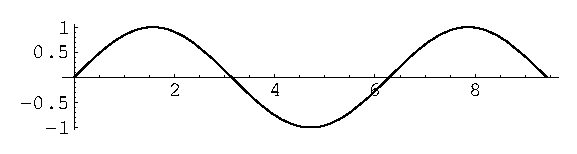
\includegraphics[width=8.5cm]{Figures/image1}}
%  \vspace{2.0cm}
  \centerline{(a) Result 1}\medskip
\end{minipage}
%
\begin{minipage}[b]{.48\linewidth}
  \centering
  \centerline{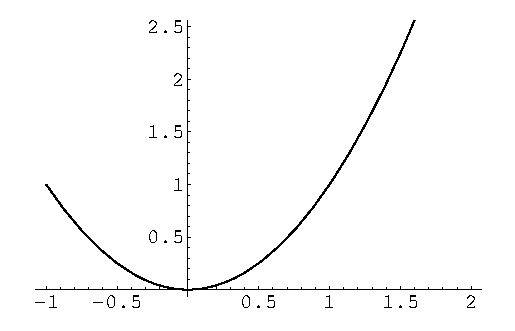
\includegraphics[width=4.0cm]{Figures/image3}}
%  \vspace{1.5cm}
  \centerline{(b) Results 3}\medskip
\end{minipage}
\hfill
\begin{minipage}[b]{0.48\linewidth}
  \centering
  \centerline{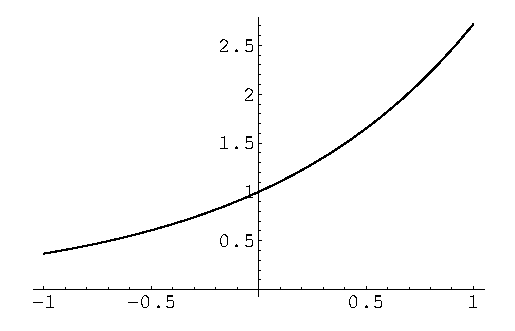
\includegraphics[width=4.0cm]{Figures/image4}}
%  \vspace{1.5cm}
  \centerline{(c) Result 4}\medskip
\end{minipage}
%
\caption{Example of placing a figure with experimental results.}
\label{fig:res}
%
\end{figure}


% To start a new column (but not a new page) and help balance the last-page
% column length use \vfill\pagebreak.
% -------------------------------------------------------------------------
%\vfill
%\pagebreak

\section{COPYRIGHT FORMS}
\label{sec:copyright}

You must include your fully completed, signed IEEE copyright release form when
form when you submit your paper. We {\bf must} have this form before your paper
can be published in the proceedings.

\section{REFERENCES}
\label{sec:ref}

List and number all bibliographical references at the end of the
paper. The references can be numbered in alphabetic order or in
order of appearance in the document. When referring to them in
the text, type the corresponding reference number in square
brackets as shown at the end of this sentence \cite{C2}. An
additional final page (the fifth page, in most cases) is
allowed, but must contain only references to the prior
literature.

% References should be produced using the bibtex program from suitable
% BiBTeX files (here: refs). The IEEEbib.bst bibliography
% style file from IEEE produces unsorted bibliography list.
% -------------------------------------------------------------------------
\bibliographystyle{IEEEbib}
\bibliography{refs}

\end{document}
